% !TeX root = ../dokumentation.tex

\addchap{\langanhang}

 

{\Large
\begin{enumerate}[label=\Alph*.]
	\item Einschwingzeit 90\% 0000 0000 -> 0000 0001
	\begin{figure}[H]
		\centering
		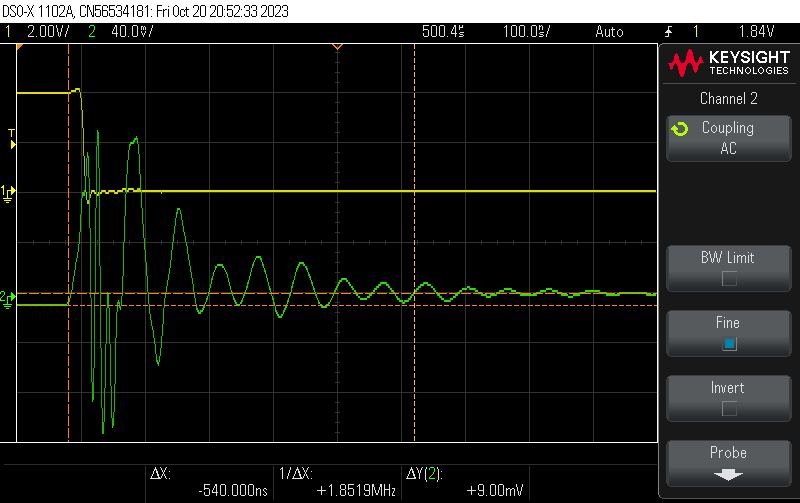
\includegraphics[height=6cm]{images/einschwingszeit00000000-00000001_90proz.png}
	\end{figure}
	\item Einschwingzeit 100\% 0000 0000 -> 0000 0001
	\begin{figure}[H]
		\centering
		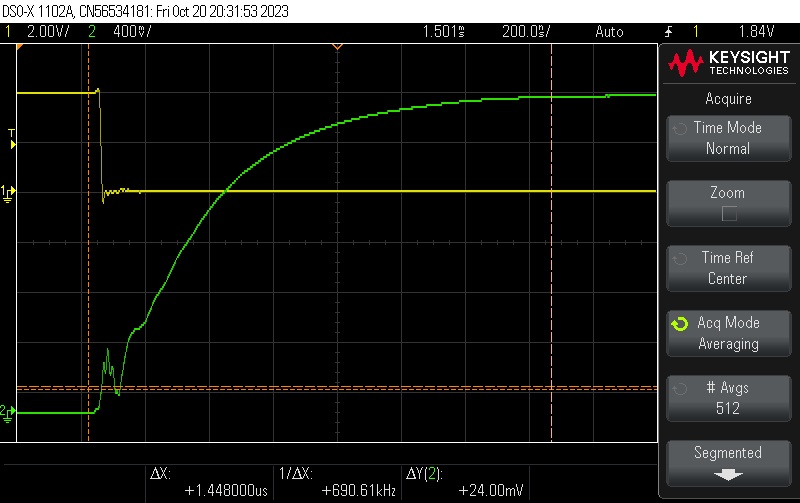
\includegraphics[height=6cm]{images/einschwingszeit00000000-11111111_100proz.png}
	\end{figure}
	\pagebreak
	\item Einschwingzeit 90\% 0000 0000 -> 1111 1111
	\begin{figure}[H]
		\centering
		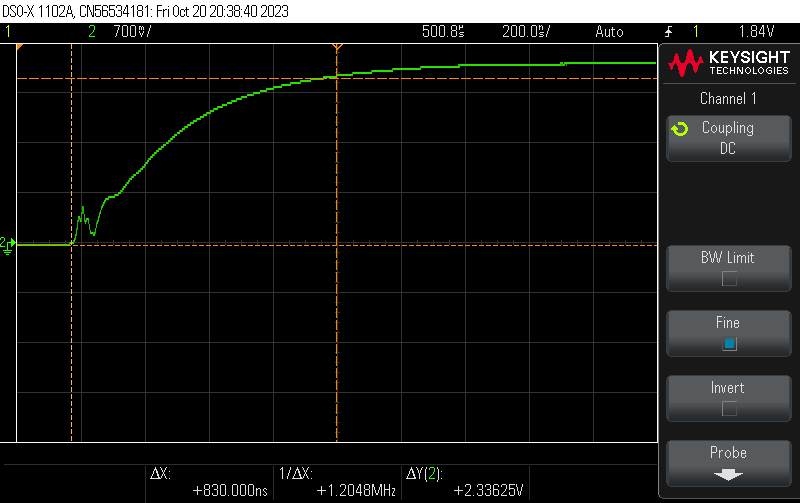
\includegraphics[height=6cm]{images/enschwingszeit00000000-11111111_90proz.png} 
	\end{figure}
	\item Einschwingzeit 100\% 0000 0000 -> 1111 1111
	\begin{figure}[H]
		\centering
		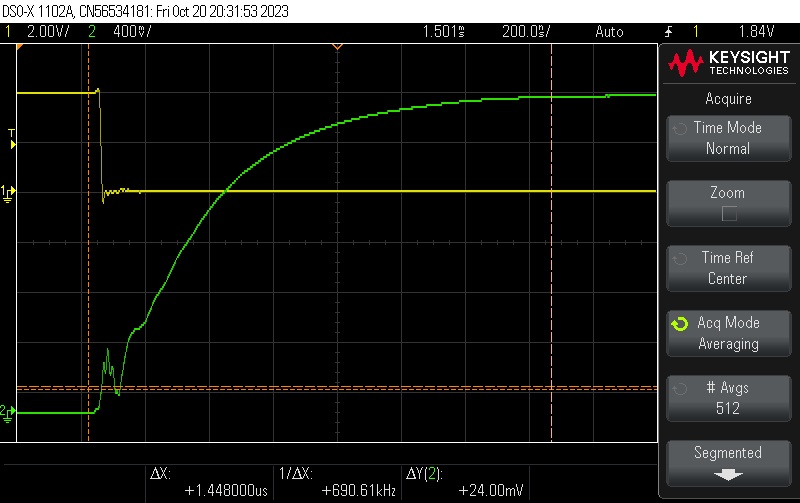
\includegraphics[height=6cm]{images/einschwingszeit00000000-11111111_100proz.png} 
	\end{figure}
\end{enumerate}
}
